\chapter{Related Work}
\label{chapter:related_work}
\begin{quote}
Prior research has leveraged expert help and demonstrations to support people learning and using creative and complex software. In this chapter, I first describe the challenges of using web search to find expert resources. Then, I discuss how different types of expert resources support the different user goals of understanding processes, achieving outcomes, and both together. Through examples of both out-of-context and in-context assistance, I highlight the benefits of presenting help and demonstrations in context, motivating the systems in this dissertation.
\end{quote}

\section{Expert Resources Abound Online but are Hard to Use}
People often need help when using complex software due to its steep learning curve \cite{Adar2014}. Most software provides some in-situ assistance and official documentation, but these are typically limited to introductory tasks and individual tool descriptions \cite{Lafreniere2014a}. As a result, people often turn to expert resources shared in online user communities, such as tutorials, discussion fora, examples, and video demonstrations. Expert resources are more abundant than ever, as they are relatively easy to make and share online \cite{Pongnumkul2011, Lafreniere2013a}. Web search provides a powerful way to quickly browse and access these resources, but it poses three key problems. First, users must articulate an appropriate query, an almost paradoxical requirement for users who are there because they don't know the domain \cite{Russell2011}. Novices often don't have enough prior knowledge to even know \textit{what} to ask, let alone how to ask it \cite{Miyake1979}. Second, search is blind to relevant contextual information that could connect users to better resources \cite{Ekstrand2011, Kraft2005, Finkelstein2002}. People must know exactly what they're looking for, or spend time looking at potentially irrelevant information. Finally, search is divorced from the application UX, requiring users to bounce back and forth to connect online resources with their own task \cite{Fourney2014Intertwine}. The systems in this dissertation bring online expert help and demonstrations into the user's context, and use contextual information to improve the relevance of the presented resources.

Searching is helpful when users know what they need, but novices often don't \cite{Miyake1979}, and starting from a blank slate can be intimidating \cite{Kelley2013}. Proactively recommending help and examples in-situ based on user context can lead users to information they might not have even thought to search for \cite{Matejka2009, Chilana2012, Matejka2011, Ichinco2017}, and can spark creative inspiration \cite{Bawden1986, Kulkarni2014, Herring2009}. All the systems in this paper therefore present \textit{something} to the user by default: LiveClips, DiscoverySpace, and CritiqueKit all recommend resources automatically based on the user's behaviour or document. RePlay and ReMap present general videos related to the current application when opened, and encourage the user to search for the tools they are using by automatically adding their names to the search field when clicked. 

The remainder of this chapter discusses relevant approaches for leveraging expert resources to help novices understand processes and achieve desired outcomes in creative or complex software. This prior work highlights the importance of presenting resources in context and using contextual information to improve their relevance and usefulness. 

\section{``I Need Help Accomplishing My Goal'': Tutorials and De\-monstrations Enable Learning While Doing}
Online tutorials, demonstrations, and walkthroughs are popular resources for users of complex software looking for procedural help. Although they tend to show an entire task from start to finish, one of the biggest reasons people seek both text \cite{Lafreniere2013a} and video \cite{AlamAnik2015} tutorials is for in-task help with a specific goal. People learning complex software often ``learn on the job,'' seeking process-related help for achieving a specific outcome (\autoref{fig:intro_designspace} top right).

Prior work has made tutorials easier to navigate and understand by allowing people to add comments and questions at specific locations in text tutorials \cite{Bunt2014} and specific timestamps and visual locations in video tutorials \cite{AlamAnik2015}, or recording multiple versions of tutorials so viewers can explore different use cases \cite{Lafreniere2013}. Video tutorials are especially helpful for learning when people are in the execution stage of creative work \cite{Zhang2019}, because they show clear demonstrations that might be harder to explain or understand in text \cite{Chi2012, Pongnumkul2011, Grossman2010a}. However, videos are harder to navigate and skim than text because because they show a single unstructured stream of information and can typically only be explored by scrubbing on the timeline with a small visual preview \cite{Pavel2014, Pavel2015, Kim2014}. Segmenting videos into conceptual chunks \cite{Pongnumkul2011, Chi2012, Banovic2012, Nguyen2015, Grossman2010a, Matejka2011} and adding navigational cues \cite{Matejka2011, Grossman2010, Kim2014, Banovic2012, Kim2014a, Pongnumkul2011, Grossman2010a, Chi2012, Pavel2014, Nguyen2015} can help viewers more easily find the information they need. Methods for navigating between video segments include interactive timeline markers \cite{Matejka2011, Grossman2010, Kim2014, Banovic2012, Kim2014a}, thumbnail images \cite{Kim2014a, Pongnumkul2011, Banovic2012, Grossman2010a, Chi2012, Pavel2014}, transcript text \cite{Kim2014a}, and clickable elements overlaid on the video \cite{Nguyen2015}. For example, ToolScape \cite{Kim2014, Kim2013} shows a clickable thumbnail image and description of the tools used for each step of the video's process, highlights areas of the video with no visible progress, and allows users to browse storyboard views of videos based on their steps (\autoref{fig:intro_toolscape}). These cues make it easier for users to quickly browse and navigate videos, and skip to or repeat relevant steps when following along, leading users to produce better work with higher self-efficacy \cite{Kim2014, Kim2013}. However, they require manually annotating videos or crowdsourcing and verifying labels.

\begin{figure}[t!]
\centering
  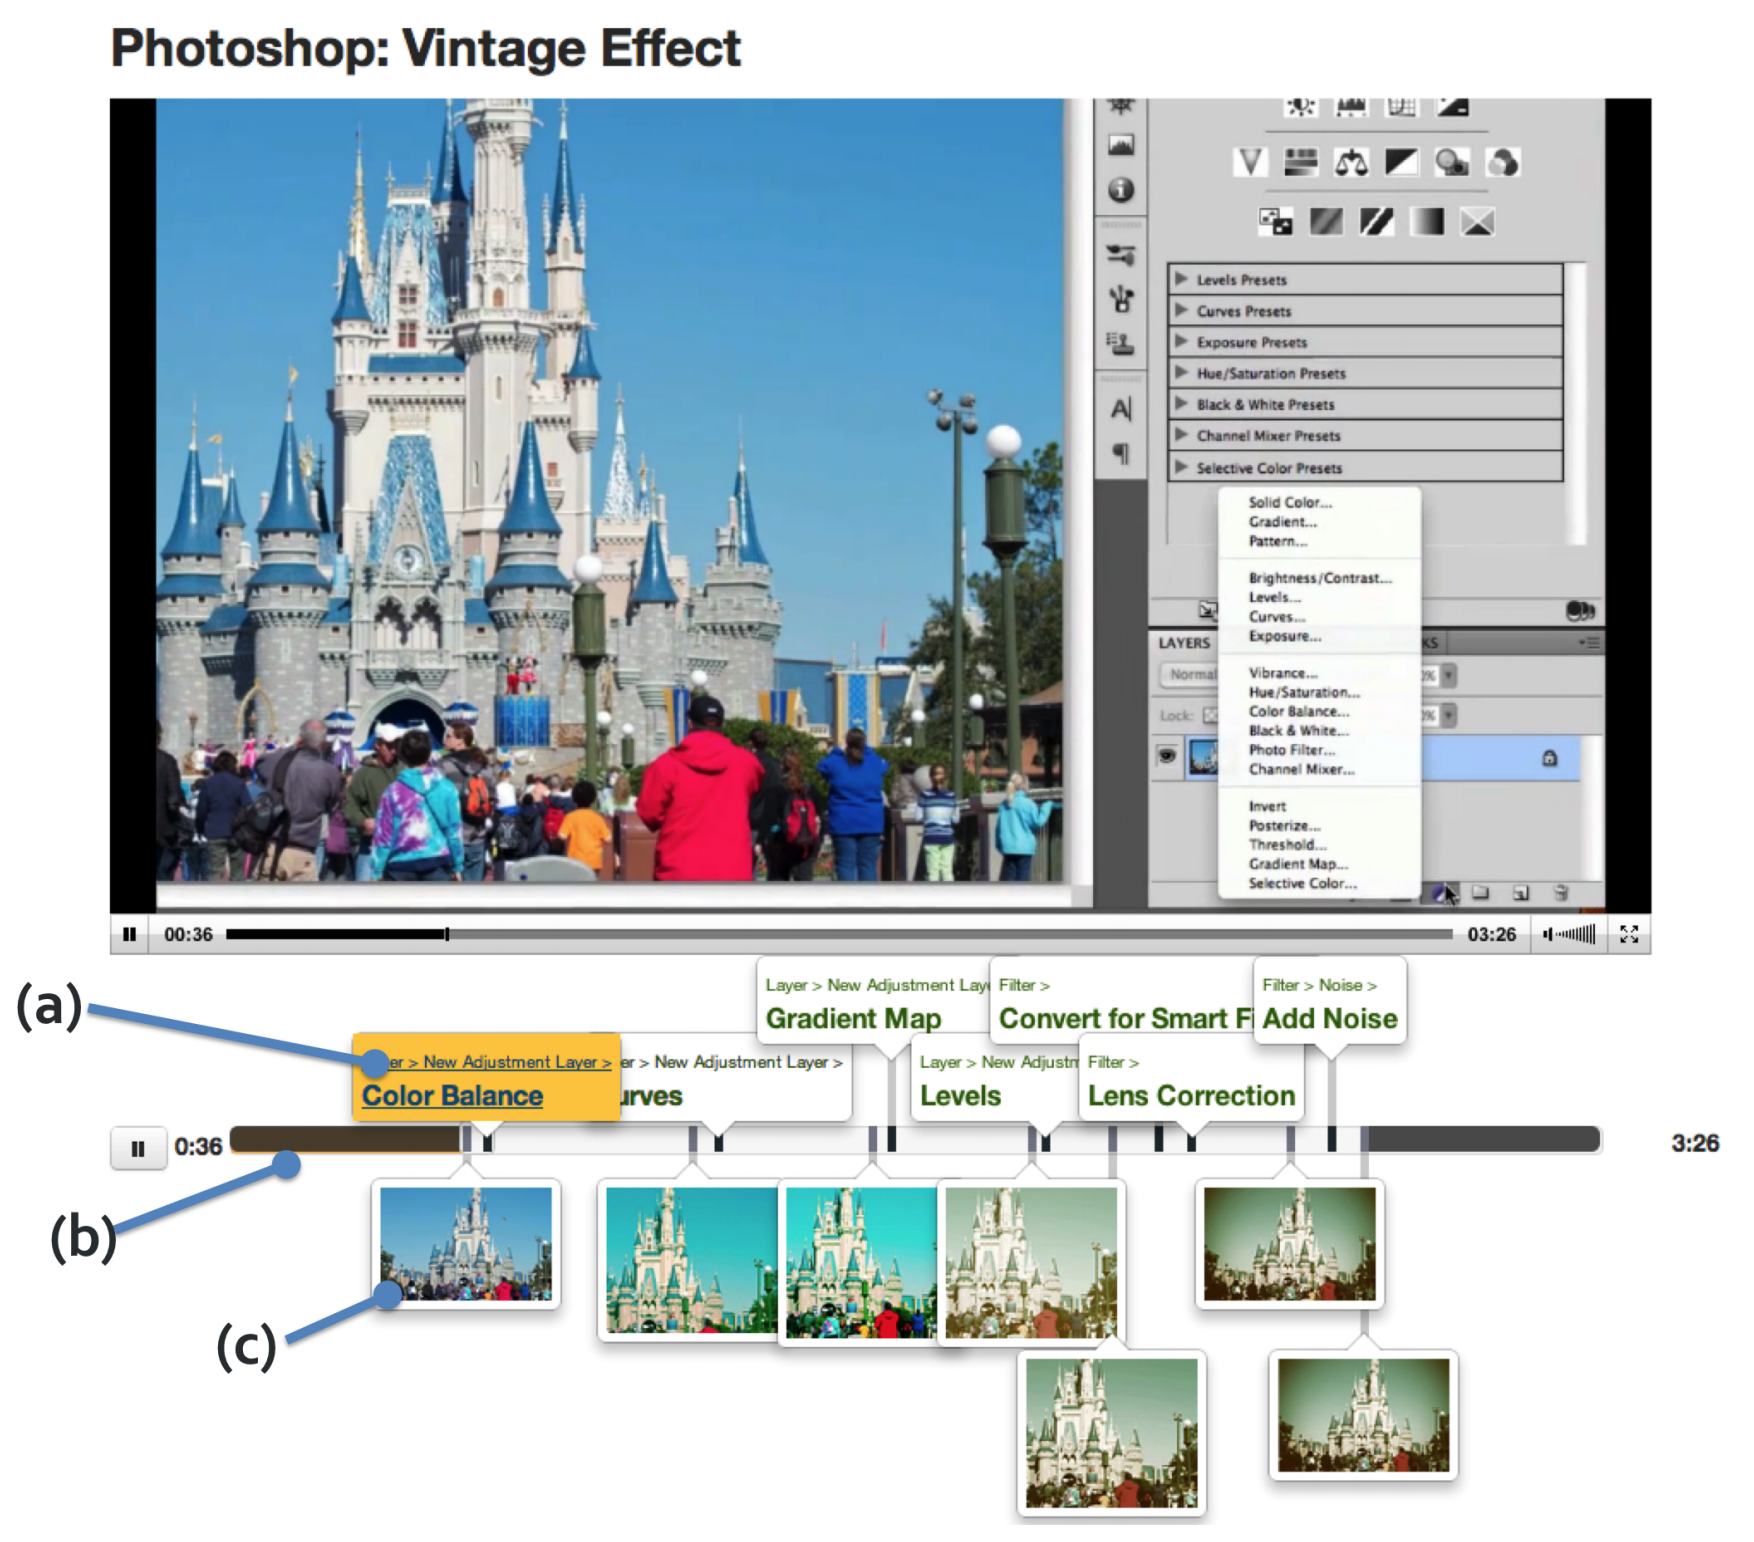
\includegraphics[width=0.7\textwidth]{figures/toolscape.png}
  \caption{ToolScape helps users follow along with video tutorials by adding clickable descriptions (a) and thumbnail images (c) for each step of the video’s process, and highlighting areas of the video with no visible progress (b). Figure originally published by Kim \textit{et al.} \cite{Kim2014}.}~\label{fig:intro_toolscape}
\end{figure}

Systems for viewing tutorials on the web (like ToolScape \cite{Kim2014, Kim2013}) require the user to find a relevant tutorial for their current task from a set of search results. One way to improve the relevance of search results is to augment web search queries with context from the user's software \cite{Ekstrand2011, Brandt2010, Matejka2011a}. Systems can also leverage user context to highlight relevant information within a result, making it easier for users to relate to their task \cite{Ekstrand2011, Fourney2014Intertwine}. But even once the user finds a relevant result, viewing it in a separate window presents difficulties such as switching back and forth between the browser and the application and mapping screenshots or videos of the application to the user's own version \cite{Kelleher2005, Pongnumkul2011}. 

Embedding learning resources in software reduces the need for context switching, and supports active learning, or learning while doing \cite{Bonwell1991, Grossman2010a, Matejka2011, Ichinco2017, Matejka2009, Greene2002}. For example, interactive tutorials guide users step-by-step through hands-on example tasks inside the target application \cite{Kelleher2005, Lafreniere2014a, Pongnumkul2011}. Such tutorials can even be generated automatically as a user demonstrates them \cite{Grabler2009}, though this requires domain-specific heuristics. In-application search for tutorials \cite{Lafreniere2014a} or question \& answer forum posts \cite{Chilana2012} also helps users stay focused on their task while seeking help. CheatSheet \cite{Vermette2015} and Social CheatSheet \cite{Vermette2017} support manual and collaborative curation (respectively) of help resources, which the systems then leverage to display relevant help in context while using web applications. Like the systems in this dissertation, CheatSheet and Social CheatSheet display help resources in a sidebar to make them easily accessible and searchable in context while completing a task (\autoref{fig:intro_cheatsheet}).

\begin{figure}[b!]
\centering
  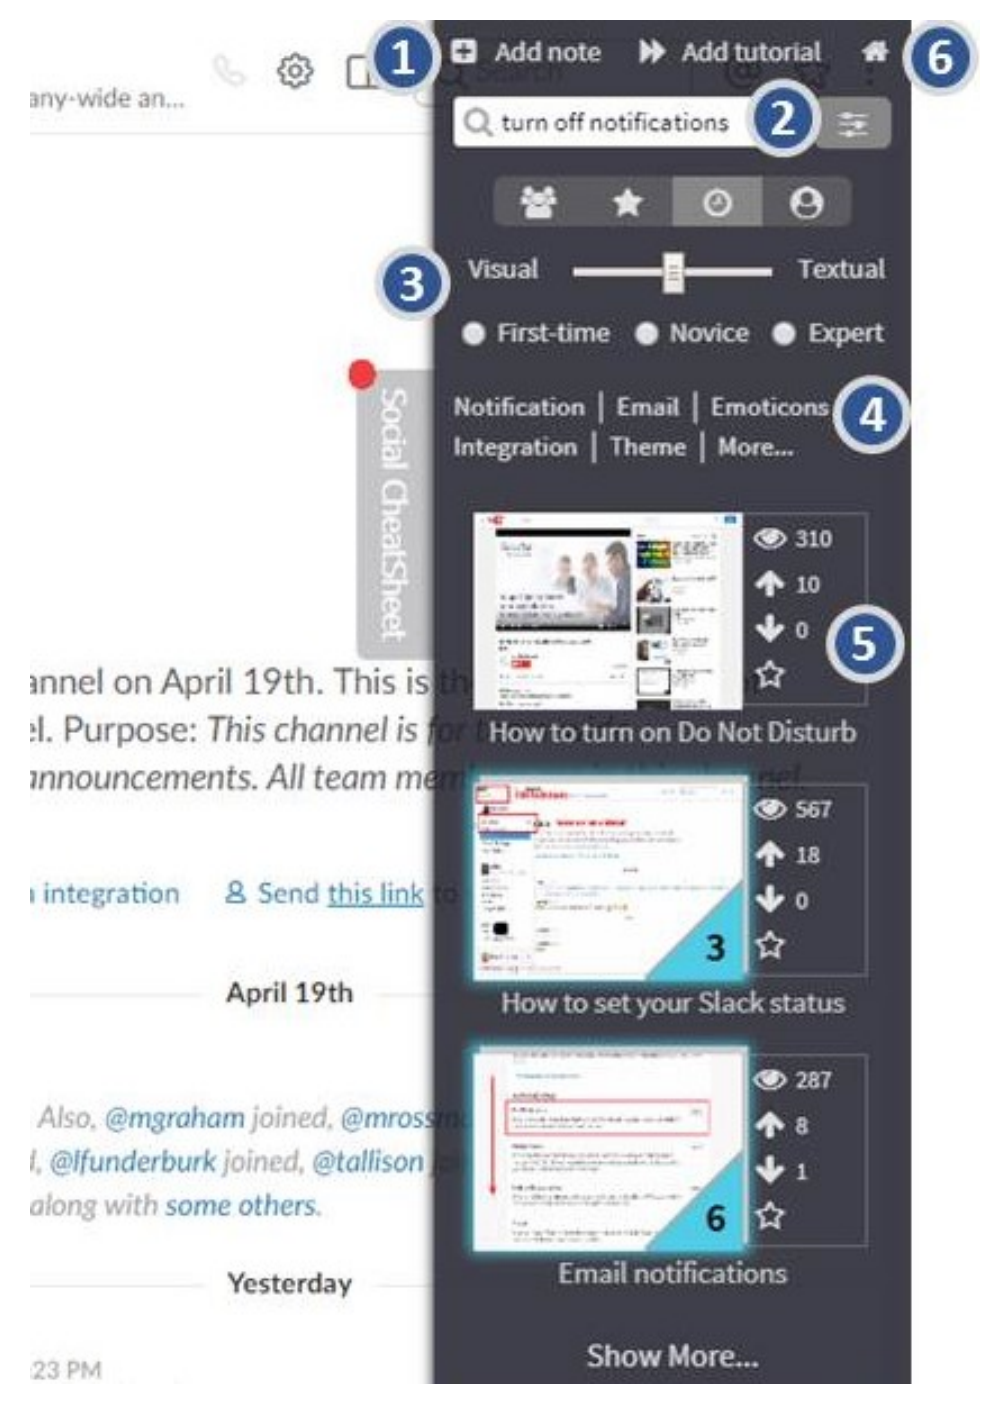
\includegraphics[width=0.5\textwidth]{figures/social-cheatsheet.png}
  \caption{Social CheatSheet displays help resources for the user's current web application in a sidebar to make them easily accessible and searchable in context while completing a task. Figure originally published by Vermette \textit{et al.} \cite{Vermette2017}.}~\label{fig:intro_cheatsheet}
\end{figure}

\section{``I Don't Know What My End Goal Is'': Proactive Suggestions Enable Discovery and Inspiration}
Besides help with specific tasks, common general-purpose uses for tutorials include learning a new topic or software, studying for a class, or shadowing an expert \cite{Lafreniere2013a} (\autoref{fig:intro_designspace} top left). Other popular resources for these goals besides tutorials include online lectures via video (\textit{e.g.}, through MOOC platforms like Coursera\footnote{\href{https://www.coursera.org/}{\nolinkurl{coursera.org}}}) or podcast (\textit{e.g.}, through platforms like iTunes U\footnote{\href{https://apps.apple.com/us/app/itunes-u/id490217893}{\nolinkurl{apps.apple.com/us/app/itunes-u/id490217893}}}), online textbooks, blogs, and live stream videos \cite{Lu2019}. People use these resources not just for learning, but also for inspiration, motivation, and entertainment \cite{Lu2018, Hilvert-Bruce2018, Lu2019, Cheung2011}.

Resources that encourage trying things out and/or discovering new features can be helpful when people are interested in process outside of a task. People sometimes tinker in software without having an explicit goal in mind, learning features by trying them out \cite{Burnett2016, Carroll1987}. To support this behaviour, interactive tutorials can help users learn and practice skills through predefined tasks \cite{Dontcheva2014, Lafreniere2014a, Kelleher2005}. Proactively suggesting related commands \cite{Li2011, Matejka2009} or videos \cite{Grossman2010a, Matejka2011} can help users discover new features that are useful for their workflows or learn about new functionalities for tools they already use. For example, ToolClips \cite{Grossman2010a} augments traditional tooltips that appear when hovering over a tool with video demonstrations of that tool being used (\autoref{fig:intro_toolclips}). They are a good example of contextual assistance that is readily available in-situ but not distracting or obtrusive; ToolClips only appear if a user pauses while hovering over a tool, and are easily dismissed by mousing away. Users can view multiple videos of each tool to see different possible uses for them. Most importantly, the videos shown are short clips that show only the tool use and its surrounding context independent from any particular task, thus steering users directly to the relevant information. 
%Like ToolClips \cite{Grossman2010a}, LiveClips is largely inspired by ToolClips \cite{Grossman2010a} in that it recommends video clips to users in context.

\begin{figure}[t!]
\centering
  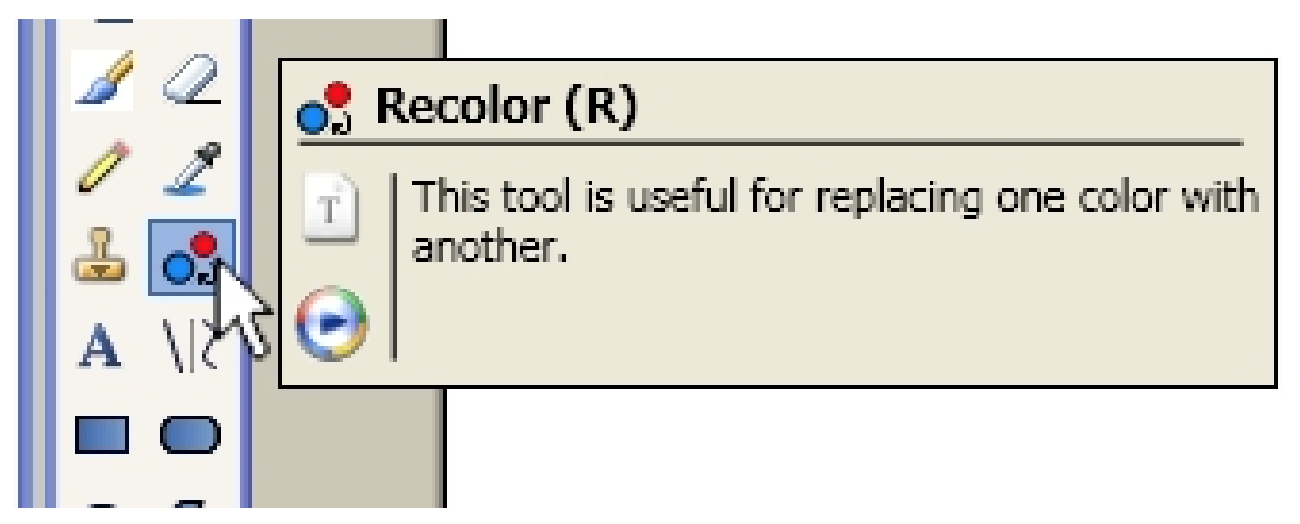
\includegraphics[width=0.4\textwidth]{figures/toolclips1.png}
  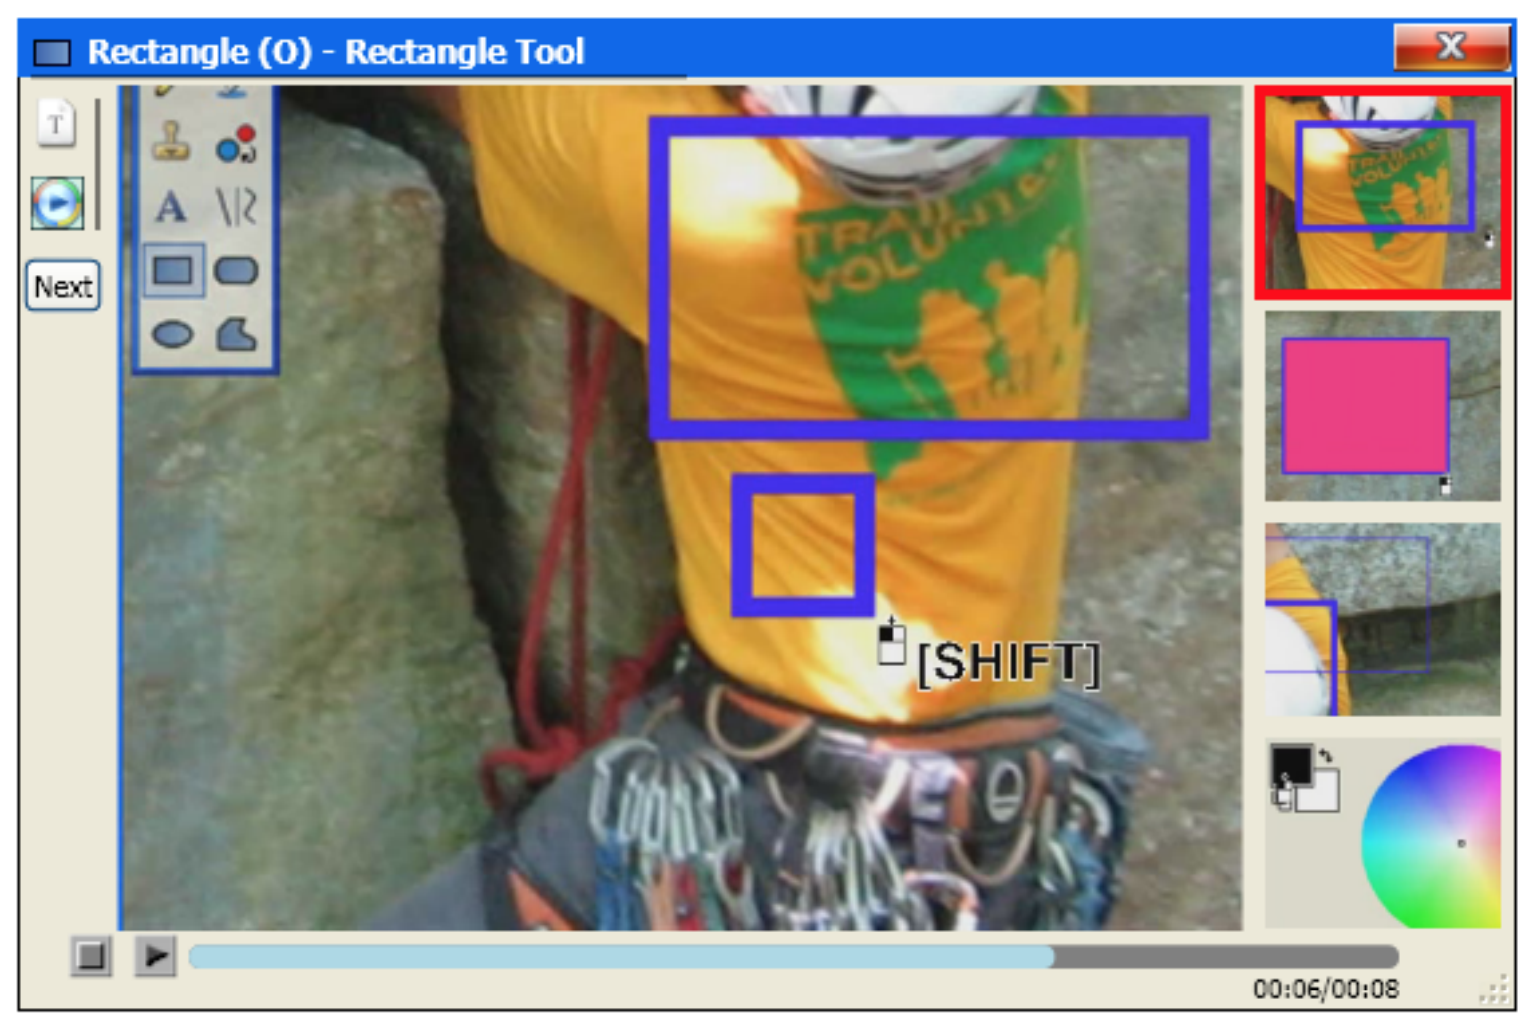
\includegraphics[width=0.5\textwidth]{figures/toolclips2.png}
  \caption[ToolClips helps users learn how to use software tools in-situ by augmenting traditional tooltips with video demonstrations. Figure originally published by Grossman \textit{et al.} \cite{Grossman2010a}.]{ToolClips helps users learn how to use software tools in-situ by augmenting traditional tooltips with video demonstrations. Clicking the media button on the tooltip (left) opens a video player (right) showing concise demonstrations of the tool being used. Figure originally published by Grossman \textit{et al.} \cite{Grossman2010a}.}~\label{fig:intro_toolclips}
\end{figure}

This prior work focuses on helping users \textit{learn} processes; what about when users seek \textit{inspiration}? Inspiration is difficult to study because its unpredictable nature and influence makes it hard to quantify \cite{Shneiderman2007}.
While inspiration can stem from just about anywhere, one proven way to stimulate creative inspiration is browsing examples of other artists' work \cite{Benjamin2014, Foster2003, Shneiderman2007, Shneiderman2002, Muller-Wienbergen2011, Greene2002, Bawden1986}. Creative work often combines preexisting works in novel ways \cite{Benjamin2014}, or draws new connections between seemingly disparate things \cite{Foster2003}. Examples can be beneficial not just at the beginning of the creative process, but throughout \cite{Kulkarni2014, Siangliulue2015, Rhodes1996}. LiveClips (Chapter \ref{chapter:liveclips}) therefore recommends video examples to users in context. Unlike ToolClips \cite{Grossman2010a}, LiveClips takes its video clips from creative live streams and aims to \textit{inspire} users rather than educate them.

\section{``I Have a Goal and Want It Done'': Operations and Answers Help People Accomplish Tasks}
Users often have high-level goals when using creative software, such as making a photo look ``better'' \cite{Laput2013}. To accomplish these goals, users must bridge the \textit{gulf of execution} \cite{Hutchins1985}, figuring out which tools to combine and how to use them in order to achieve their goal. Sometimes, people don't have the time or patience to learn the details of each tool required -- they simply want to get a task \textit{done} \cite{Laput2013, Manuvirakurike2018} (\autoref{fig:intro_designspace} bottom right). 

The classic solution when one wants to get a task done but doesn't know how would be to ask a friend to do the task for you or provide help. Or, if you don't know who to ask, systems like Answer Garden \cite{Ackerman1990} could automatically route a question to an appropriate expert for answers. On the web, people seek answers or results from experts by posting questions in discussion fora such as StackOverflow or requests in fora such as \href{https://www.reddit.com/r/PhotoshopRequest/}{\nolinkurl{r/PhotoshopRequest}} on Reddit \cite{Manuvirakurike2018}. However, questions asked on the web lack the context that is normally available when seeking help in-person, such as system settings or details about what the user has already tried \cite{Asaduzzaman2013, Chen2017}. Looking through previously-answered questions on discussion fora can help people find solutions without needing to post a new question, but reading through past discussions to find a single relevant answer is tedious and requires users to know what keywords they are looking for \cite{Chilana2012}. 

% \begin{figure}[b!]
% \centering
%   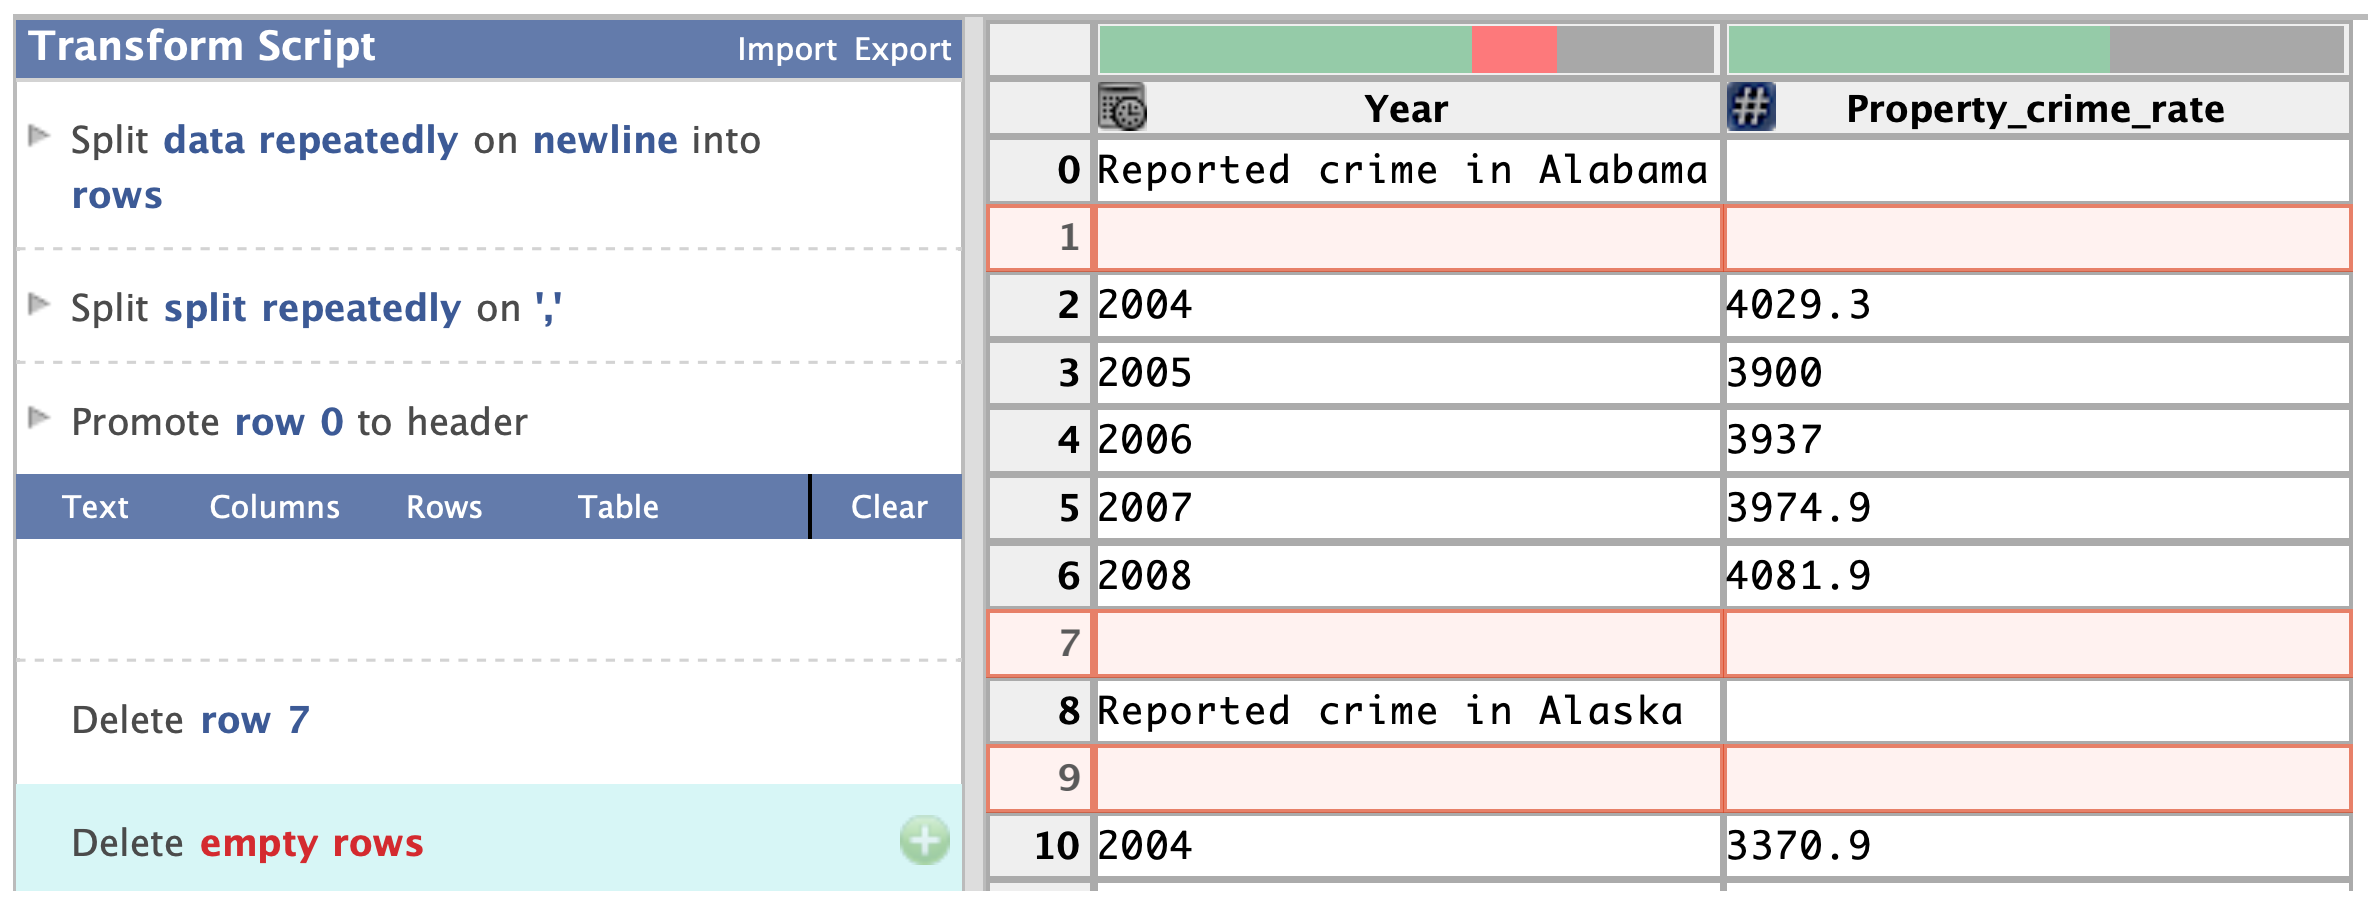
\includegraphics[width=0.9\textwidth]{figures/wrangler.png}
%   \caption{Wrangler suggests relevant data transforms (bottom left) to help users clean up large datasets (right) more efficiently. Suggestions update in response to user actions, and clicking the ``add'' button next to a suggestion applies it automatically. Figure originally published by Kandel \textit{et al.} \cite{Kandel2011}.}~\label{fig:intro_wrangler}
% \end{figure}
\begin{figure}[b!]
\centering
  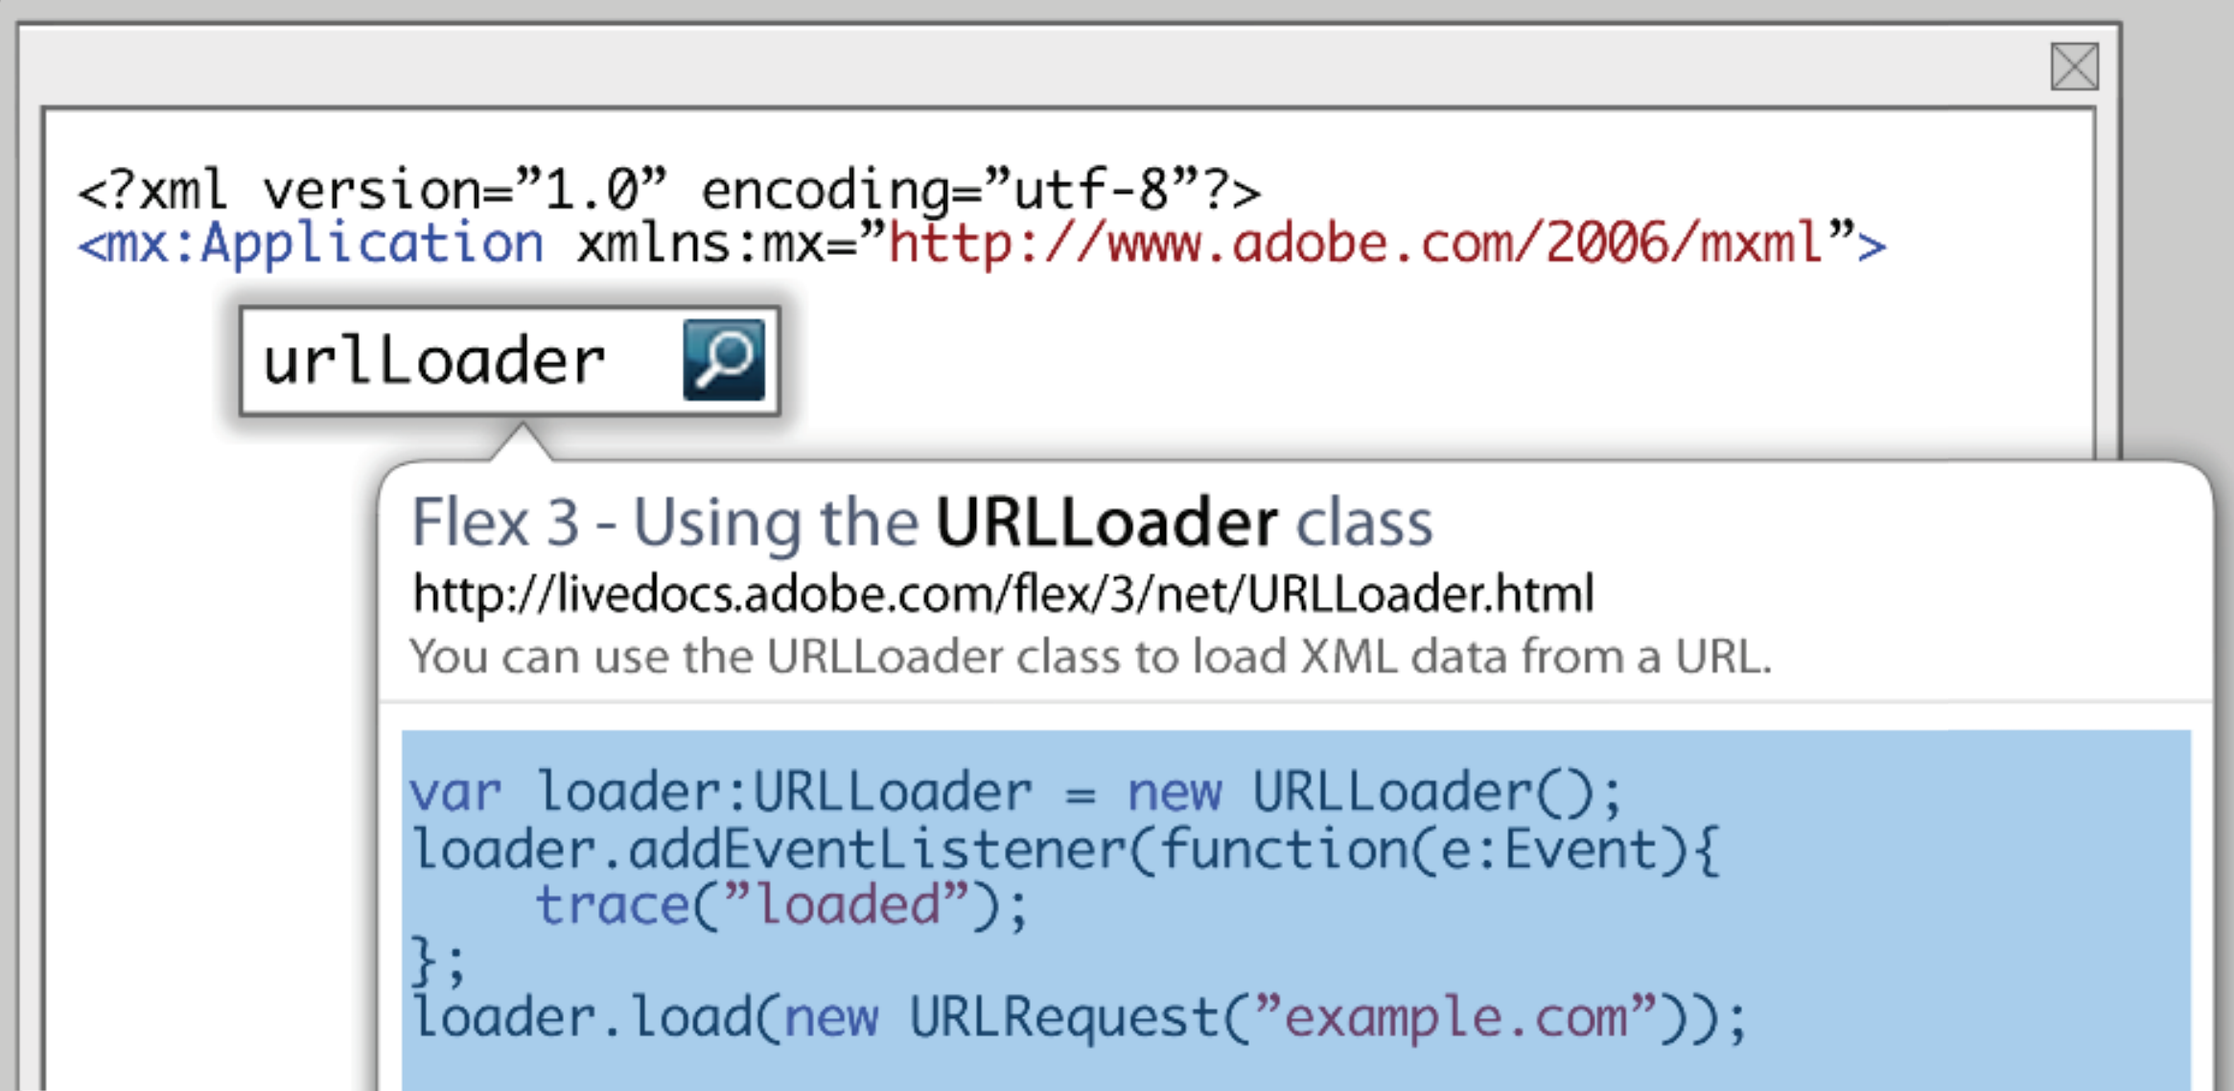
\includegraphics[width=0.49\textwidth]{figures/blueprint1.png}
  \hfill
  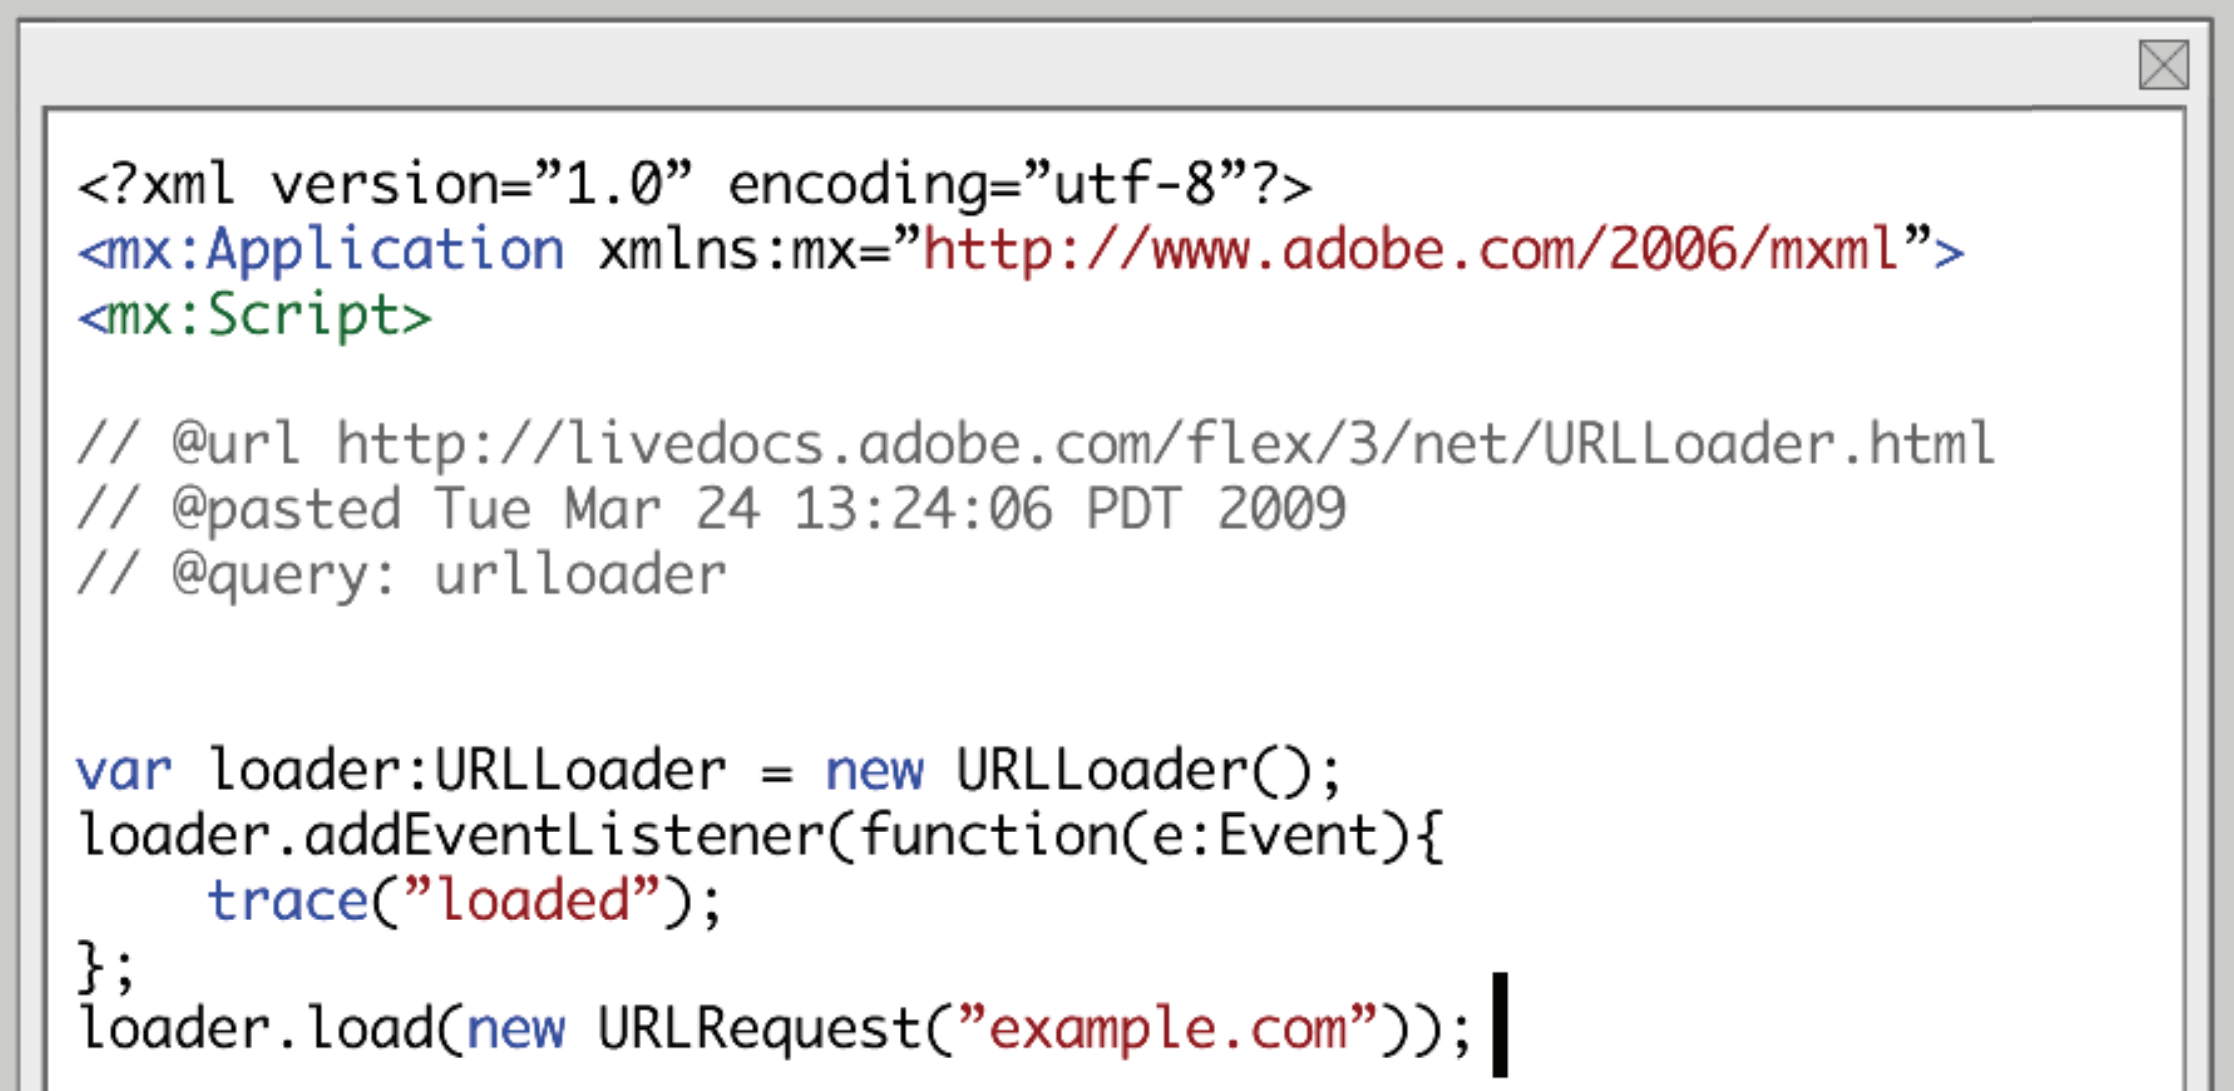
\includegraphics[width=0.49\textwidth]{figures/blueprint2.png}
  \caption{Blueprint enables in-context search and use of code examples from the web. It extracts code snippets from web pages (left) and allows users to integrate them into their code in one click (right).  Figure originally published by Brandt \textit{et al.} \cite{Brandt2010}.}~\label{fig:intro_blueprint}
\end{figure}

One way to bring question-asking into the user's context and ensure that relevant information is included is to have users record their question directly in the application \cite{Chen2017}. Another is to embed discussion fora directly into the application, allowing users to narrow down questions based on relevant interface elements \cite{Chilana2012} or recently-used commands \cite{Matejka2011a}. To achieve outcomes even more directly than by question and answer, other systems embed contextual search or suggestion of resources such as reusable examples \cite{Brandt2010}, executable operations \cite{Kandel2011}, solutions to errors \cite{Hartmann2010}, and software features \cite{Adar2014}. Presenting such resources in context allows users to apply them directly to their work without having to stop their task, and allows systems to improve the relevance of results by leveraging contextual information. 
For example, Blueprint \cite{Brandt2010} enables in-context search of example code to help programmers more easily integrate code from the web into their own tasks (\autoref{fig:intro_blueprint}). Blueprint extracts code examples from existing web resources, presents them in context, and allows users to instantly apply them to their own code. Blueprint also augments search queries with relevant context from the user's environment to find more relevant results.
%For example, Wrangler \cite{Kandel2011} suggests relevant data transforms to help users clean up large datasets more efficiently (\autoref{fig:intro_wrangler}). Wrangler generates suggestions by comparing the user's actions to a corpus of previous usage data and identifying likely transforms. Users can then select a transform to apply it directly to their dataset, removing the need to write complicated scripts or do tedious manual cleaning. 
Like Blueprint, DiscoverySpace (Chapter \ref{chapter:discoveryspace}) and CritiqueKit (Chapter \ref{chapter:critiquekit}) suggest reusable examples in context to help users achieve better outcomes more easily.
